\documentclass[12pt]{article}
\usepackage{geometry}
\usepackage[english]{babel}
\usepackage[utf8]{inputenc}
\usepackage{fancyhdr}
\usepackage{graphicx}
\usepackage{titlesec}


\setlength{\headheight}{15.2pt}
\setcounter{secnumdepth}{4}

\titleformat{\paragraph}
{\normalfont\normalsize\bfseries}{\theparagraph}{1em}{}
\titlespacing*{\paragraph}
{0pt}{3.25ex plus 1ex minus .2ex}{1.5ex plus .2ex}

\rfoot{Pg: \thepage}

\geometry{
   a4paper,
   left = 20mm,
   top = 20mm,
}
\begin{document}
\thispagestyle{empty}

\section*{}
{\LARGE\makebox[\textwidth]{\textbf{KATHMANDU UNIVERSITY}}}

\centerline{Department of Computer Science and Engineering}
\centerline{Dhulikhel,Kavre}
\begin{figure}[h]
    \centerline{
\includegraphics[width=50.546mm,height=50.546mm]{KU_Logo.png}}
\end{figure}

\centerline{\textbf{A Project Report}}
\centerline{on}
\centerline{\underline{\textbf{"Covid-19 Situation Analysis Application"}}}

\vspace*{12mm}

\centerline{\textbf{[Code No. : COMP 206]}}
\centerline{(For partial fulfillment of 2nd Year/ 3rd Semester in Computer Science)}

\vspace*{10mm}

\centerline{\textbf{Submitted by}}
\centerline{\textbf{Aayush Pokharel(Roll No. 43)}}
\centerline{\textbf{Dikshya Poudel (Roll No. 45)}}
\centerline{\textbf{Sajag Pradhanang (Roll No. 47)}}
\centerline{\textbf{Samjhana Bhusal (Roll No. 60)}}

\vspace*{16mm}


\centerline{\textbf{Submitted to}}
\centerline{\underline{\textbf{Project Cordinator}}}
\centerline{\textbf{Nabin Ghimire}}
\centerline{\textbf{Dept of Computer Science and Engineering}}
\vspace*{10mm}

\centerline{\textbf{Submission Date: 13th August, 2021}}

\clearpage
\thispagestyle{empty}
\vspace*{10mm}
\centerline{\textbf{\LARGE{Bonafide Certificate}}}
\vspace*{30mm}
\centerline{\textbf{\Large{This project work on “Canteen Management System” is the}}} 
\vspace*{2mm}
\centerline{\textbf{\Large{bonafide work of}}}
\vspace*{2mm}
\centerline{\textbf{\Large{"}}}
\centerline{\textbf{\Large{Aayush Pokharel(Roll No. 43)}}}
\centerline{\textbf{\Large{Dikshya Poudel (Roll No. 45)}}}
\centerline{\textbf{\Large{Sajag Pradhanang (Roll No. 47)}}}
\centerline{\textbf{\Large{Samjhana Bhusal (Roll No. 60)}}}
\centerline{\textbf{\Large{"}}}
\vspace*{2mm}
\centerline{\textbf{\Large{who carried out the project work under my supervision.}}}
\vspace*{30mm}
\textbf{\Large{Project Supervisior}}
\\\\
\\\\
\textbf{-----------------------------------------------}
\vspace*{2mm}
\\
{\textbf{\Large{Name: Santosh Khanal}}}
\vspace*{2mm}\\
{\textbf{\Large{Assistant Professor}}}
\vspace*{2mm}\\
{\textbf{\Large{Department of Computer Science and Engineering}}}

\clearpage
\thispagestyle{empty}

\textbf{\Large{Acknowledgement}}
\vspace*{5mm}

We wish to express our sincere thanks to the Department of Computer Science and Engineering for including the COMP 206 project into our curriculum. We would like to express 
our heartfelt gratitude to our project coordinator Mr. Nabin Ghimire and our supervisor Mr. Santosh Khanal for their regular guidance and encouragement throughout the project. 
Taking this opportunity, we would like to thank all those individuals who directly or indirectly helped us in making this project successful one be it by encouraging us 
throughout the project or else through their valuable suggestions which we have tried our best to assimilate within our work.


\clearpage
\thispagestyle{empty}

\section*{Abstract}
The project ‘Covid-19 Situation Analysis Application’ proposal is drafted to meet the prerequisites to partially fulfill the COMP 206 course offered by the 
Department of Computer Science and Engineering at Kathmandu University and to cover for the pitfall of previously proposed Project ‘Portfolio Management and 
Finance Management Application’ . This project is designed to overcome the lack of centralized facility to deeply analyse COVID-19 situational data on international 
and national level. We, the involved project members, have decided to create a compact application that can run on Windows platform which scrapes data from multiple sites 
like worldometer.info, mohp.gov.np, covidnepal.org, covid19.wh.int allowing us to work on the dataset and plot various diagrams and charts necessary for in 
depth demographic analysis. It will allow customizing the charts based on demographic factors and also present trends before,
during and after a major wave. We are accomplishing this project by using dynamically typed object oriented programming language(Python) and Qt framework to handle the GUI 
portion of the application, Selenium and Scrapy to scrape web data, pandas for handling dataset and matplotlib to finally plot the data. The main goal of this 
project is to develop an efficient set of python code that can stand up to real world scenarios while increasing the programming skill of involved project members in hope 
of tackling harder projects in the forthcoming days.
\\\\
\textbf{Keywords:} Python,Qt framework, Selenium, Scrapy

\clearpage
\thispagestyle{empty}
\tableofcontents

\clearpage
\thispagestyle{empty}
\listoffigures

\clearpage
\pagenumbering{arabic}
\section{CHAPTER 1: INTRODUCTION}

\subsection{Background}
COVID-19 pandemic is a global problem which has led to a dramatic loss of human life worldwide and presents an unprecedented challenge to public health, food systems and the world of work. It has stifled the global economy, caused untold amounts of grief among family members and friends, and forced people into social 
distancing and lockdown as means of virus transmission prevention. 
\\\\
Compared to some other countries, Nepal was still in a better situation during the first wave of the pandemic but during the second wave,it was hit quite worse. The lack of accessible and accurate information have caused people to be unaware of Covid-19 risks and the need to protect themselves, get tested and vaccinated. The crisis, illness, death and isolation have increased the vulnerability of the population as a whole.
\\\\
There are few available sites that publish information on the covid situation but any data required for an in depth analysis based on different demographic factors 
are needed to be sourced from different websites. The lack of standardization of data between different websites causes cross referencing to be very difficult. To 
challenge this difficulty, we are aiming to make an open source program that is available to everyone with no cost overhead for operation. This system will be used 
by end users for the purpose of analyzing the COVID-19 situation on an international as well as on national level based on various demographics. Furthermore, this application shall also report on the availability of medical infrastructures available in Nepal to COVID-19 patients based on geographical region.

\vspace*{5mm}
\subsection{Objectives}
The main objective of this project is to understand the intermediate concepts of dynamically typed language and web scraping for enhancing our knowledge to solve 
real life problems using an Object-oriented paradigm. Besides, the other objectives are listed below:
\begin{itemize}
    \item To make various configurable graphs of multiple demographic indicators to facilitate technical analysis.
    \item To make an app which can keep people updated about the COVID-19 situation at local,national and international level. 
    \item To create a database that allows user to know about the current medical facilities near them.     
\end{itemize}

\vspace*{5mm}
\subsection{Motivation and Significance}
Our project is particularly inspired by various sites like Worldometer and covid19.mohp.gov.np. This program is being designed with an aim of collecting data that 
are available on different sites with our prior experience of the struggle of getting information in an intuitive manner. This will present a relevant user interface 
which provides easy, enjoyable and effective interaction between the user and the application along with the explanation of various graphs and their trends. Most 
notably, it will allow for analysis of transmission and mortality trends with cross reference to health infrastructures via line graph, making it more accessible 
for in depth understanding of the pandemic situation to a person untrained in technical analysis. Furthermore, this program presents features such as Vaccine 
development situations, local governmental updates, etc to facilitate understanding about the pandemic among users as a means to combat its spread.

\clearpage

\section{CHAPTER 2: RELATED WORKS}
There are similar sites available which are being used globally as well as nationally which are being operated by different NGO and governmental organizations and 
to keep track of the COVID-19 pandemic.
\\\\
Some of such sites that are in use are:

\subsection{worldometer.info}
\begin{figure}[h]
    \centerline{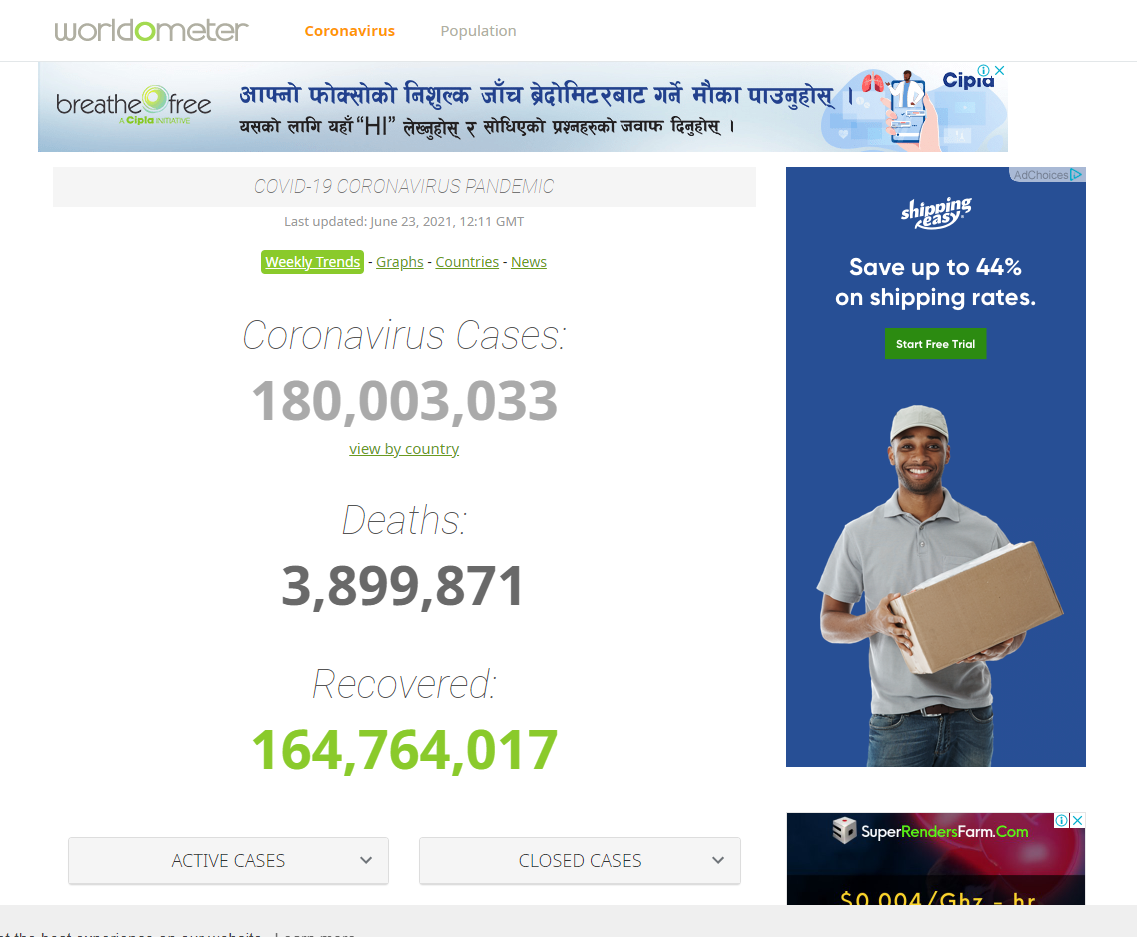
\includegraphics[width = 90mm]{worldometer.png}}
    \caption{Worldometer Website}
    \label{fig}
\end{figure}
Worldometer is a website which manually analyzes, validates, and aggregates data from thousands of sources in real time and provides global COVID-19 live statistics for a wide audience of caring people around the world. It's sources include official websites of Ministries of Health or other Government Institutions and Government authorities' social media accounts. It collects and processes data around the clock, 24 hours a day, 7 days a week and performs multiple updates per minute. 
\vspace{10mm}
\clearpage
\subsection{covid19.mohp.gov.np}
\begin{figure}[h]
    \centerline{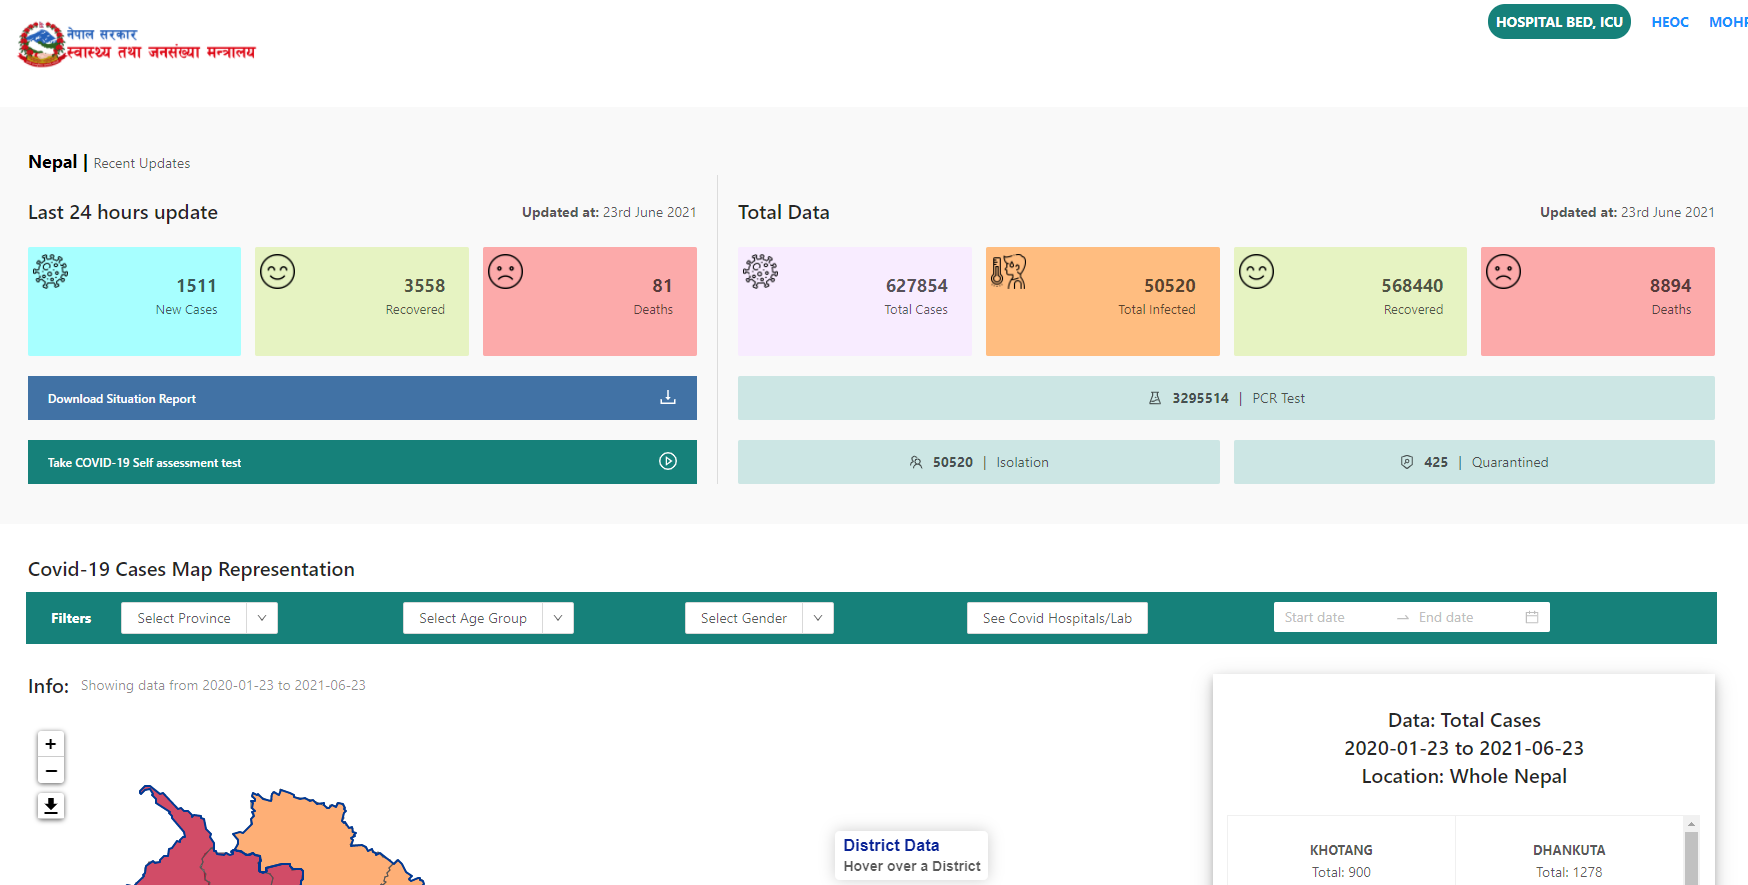
\includegraphics[width = 90mm]{mohp.png}}
    \caption{Ministry of Health and Population Website}
    \label{fig}
\end{figure}
It is an official website of Ministry of Health and Population (MoHP) designed to provide authentic information about covid situation in Nepal. It consists of all the covid related data like active cases, death cases, recovered cases classified on the basis of district, province, age, sex and compares them . It also provides information about the hospital bed availabilty for different regions to help people find proper care in time. 
\subsection{covidnepal.org}
\begin{figure}[h]
    \centerline{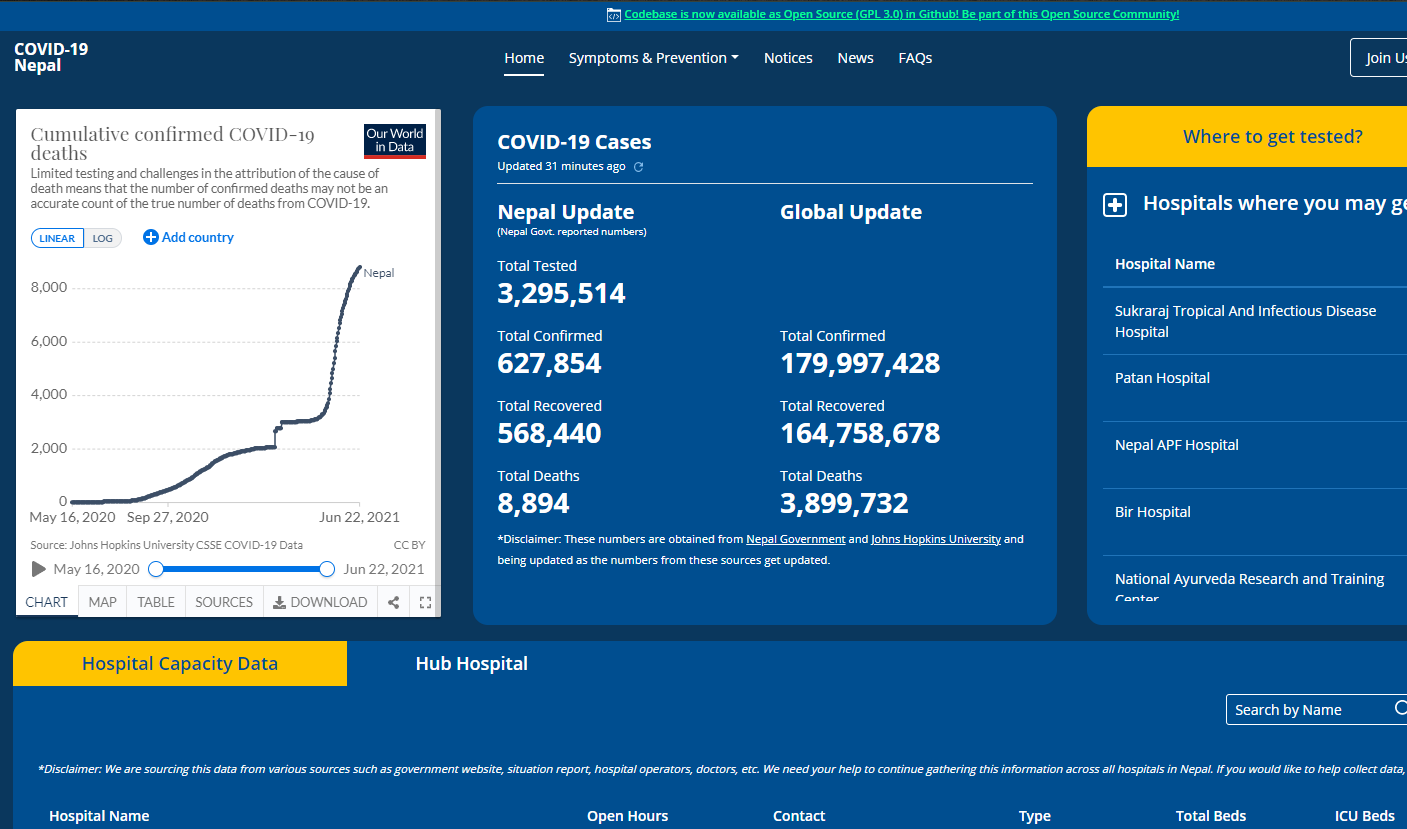
\includegraphics[width = 90mm]{covidnepal.png}}
    \caption{CovidNepal.org Website}
    \label{fig}
\end{figure}
It is an open source platform that provides reliable information about Covid-19 in Nepal along with global cases update. It also provides a general information about where and when to get tested and covid hospitals for a particular region in Nepal to get admitted along with the information about its symptoms and prevention methods. 
\clearpage

\section{CHAPTER 3: DESIGN AND IMPLEMENTATION}
\subsection{Architectural Design}

\subsubsection{Flow Chart}
\begin{figure}[h]
    \centerline{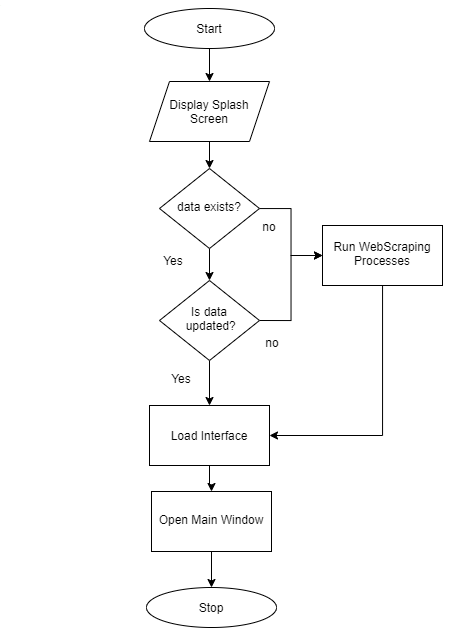
\includegraphics[width = 90mm]{SplashScreenFlowChart.png}}
    \caption{SplashScreen FlowChart}
    \label{fig}
\end{figure}
This flowchart shows the inner working of the Splash Screen Logic of the program. It checks if various data files are present and are upto date. If it doesn't find it, it runs the necessary Webscraping processes to scrape the data.
\clearpage
\begin{figure}[h]
    \centerline{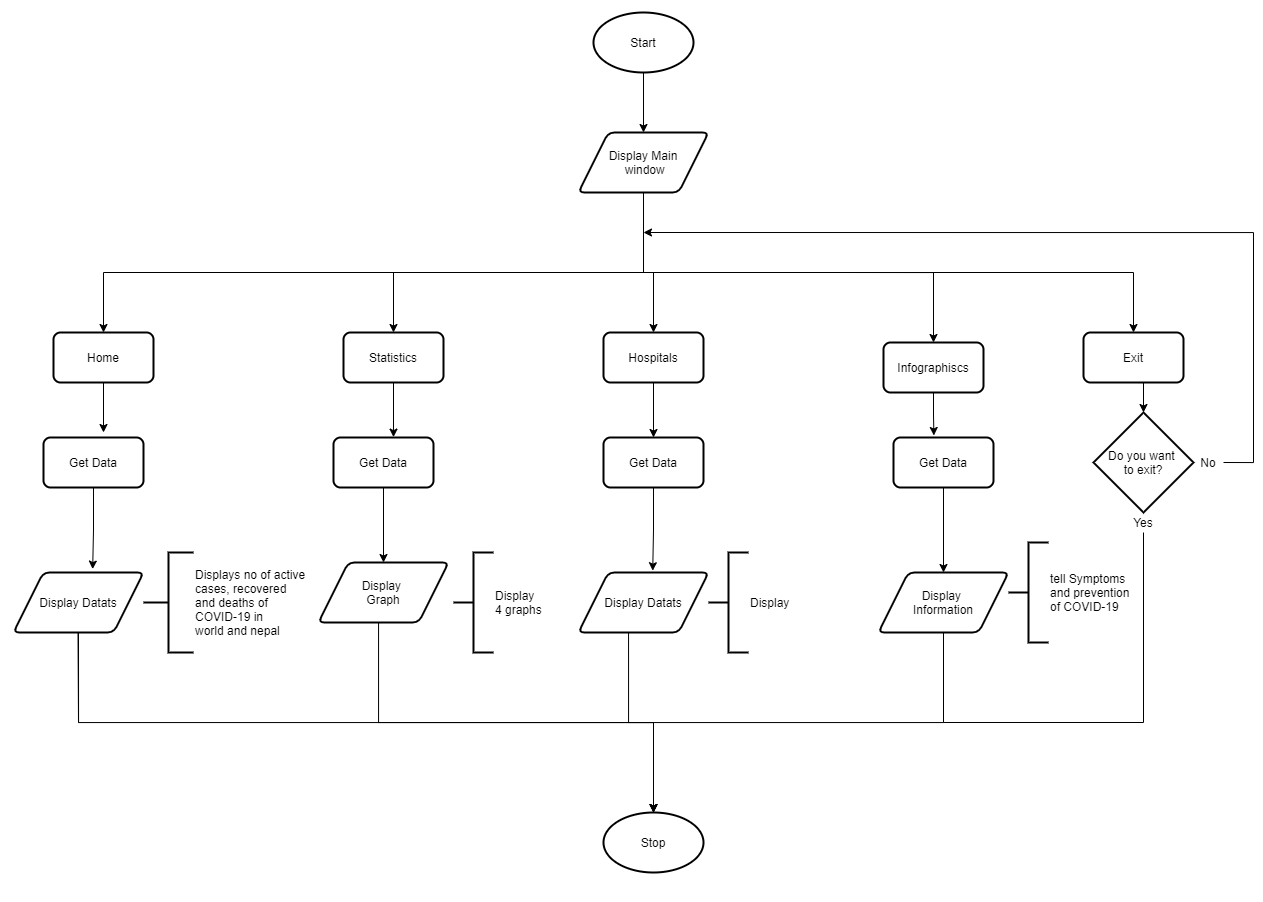
\includegraphics[width = 150mm]{MainScreenFlowChart.png}}
    \caption{MainScreen FlowChart}
    \label{fig}
\end{figure}
This flowchart shows the inner working of the Main Window and the logic of the program when user interacts with the GUI. It displays and updates graphs, charts, tables based on filters configured by the user. 
\clearpage
\subsubsection{Use Case Diagram}
\begin{figure}[h]
    \centerline{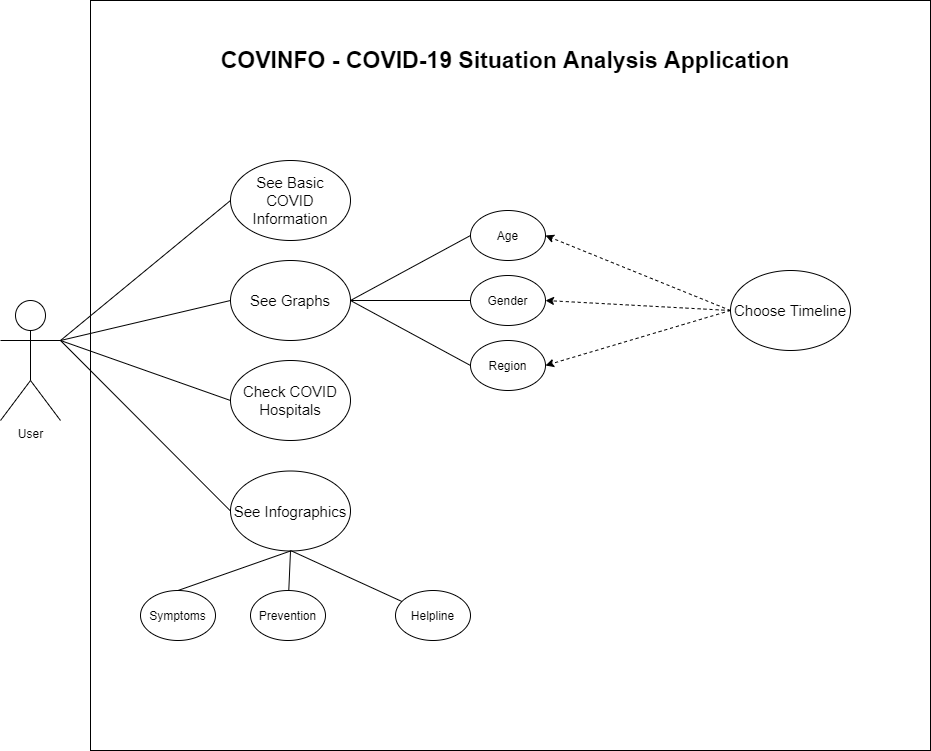
\includegraphics[width = 90mm]{UseCase Diagram.png}}
    \caption{UseCase Diagram}
    \label{fig}
\end{figure}
This use case diagram illustrates the various UI elements and its functions on Main Window of the application.

\clearpage
\subsection{System Requirement Specification}
\subsubsection{Software Requirements:}
\begin{itemize}
    \item \textbf{Front End Tools}
        \begin{itemize}
            \item The program is created using Python.
            \item Development Tools : QT frameworks
        \end{itemize}
    \item \textbf{Back End Tools}
        \begin{itemize}
            \item Selenium and Scrapy modules used for scraping web information.
            \item Pandas module used to make datasets.
            \item Matplotlib and QTGrapgh used for plotting.
            \item Web Browser supporting Selenium WebDriver \textit{(Here, Google Chrome v92.0.4515.131)}
        \end{itemize}
\end{itemize}

\subsubsection{Hardware Requirements:}
\begin{itemize}
    \item Compatibility: Compatible with all PCs running on Windows platform.
\end{itemize}

\vspace*{10mm}
\textbf{Python :} A dynamically typed multi paradigm general purpose programming language.
\\\\
\textbf{QT frameworks :} An open source cross platform multi language widget toolkit that helps in developing GUI Application.

\clearpage
\section{CHAPTER 4: DISCUSSION AND  ACHIEVEMENT}

\subsection{Methodology}
The whole process of developing the software has been divided into following aspects:
\begin{itemize}
    \item Research and study
    \item UI Design and prototyping
    \item Core programming
    \item Program Testing
    \item Documentation
\end{itemize}

\subsubsection{Research and Study}
This project being the first of the kind we have ever done, we decide to choose a subject matter that we clearly know and have experience with ie. the plotting graph 
using matplotlib. We have interacted with the various software/sites mentioned above in chapter 2 on a semi-regular basis and have experienced its strength 
and pitfall. We are trying to compile the information on nation and international stagee and present it on a singular platform.

\subsubsection{UI design and Prototyping}
The initial designs are sketched on A4 papers by our members and shared on group chat for peer review and then use QT Creator’s design tab to stub test the look 
of our UI before adding any functionality to the various widgets.

\subsubsection{Core Programming}
The most amount of project time is going to be spent in this stage. We are using the Python language to write our program. QT framework provides the necessary 
tools to create the GUI. Selenium is being used to surf the web and get html of webpages and scrapy is being used on the html file to parse and extract data 
which is converted into datasets via Pandas for easy import and manipulation as per end user requirement; for instance, getting data of certain dates only. 
Finally the QTGraph and matplotlib library is used to plot the dataset.
\paragraph{Issues Encountered}
\begin{itemize}
    \item \textit{\textbf{Change of project halfway}}\\
        The project was after the initial project was not upto par with our Supervisior. Since more than half of the work was already completed in the initial project,
        starting anew on a different topic was difficult to adjust. 
    \item \textit{\textbf{Deciding which UI language to use (QML or Qt XML)}}\\
        Due to the confusing nature of multiple libraries providing python binding for QT, we had problems choosing the approach to build the User interface. Initially we tried with
        QML to have dynamic and easily configurable UI for easier iteration but due to different OS platform present in team members' PC, getting there was version mismatch of the available 
        library between each team members. Next we tried with PySide6 but due to lack of support for Matplotlib embedding, we ultimately had to choose PySide2. 
    \item \textit{\textbf{Python library Setup}}\\
        Due to lack of proper experience in working with Command Line Interface, Team members needed to be brought up to knowledge regarding python virtual environments and pip along with teaching relevant
        commands in Powershell and Bash.
    \item \textit{\textbf{Brainstorming features to be added}}\\
        Initially the project was on different trajectory and due to amount of time invested, team members were locked in a certain direction. When the project topic was changed, the team had great difficulty in
        comming up with new ideas.
\end{itemize}
\subsubsection{Program Testing}
Unit testing was done as soon as we completed the code of a single widget to check its functioning properly. This was repeated multiple times during the development 
period to create a robust system and once the core programming is completed, alpha testing was done to find different types of bugs or ill optimised issues.
\paragraph{Bugs found and Debugged}
\begin{itemize}
    \item Graph wasn't being updated when the timeline was being changed.
    \item Program was loading old data files in Splash screen instead of running scraping command.
    \item Scrapy wasn't making files in proper location after scraping was complete.
    \item Blank information was being scraped from the website of MOHP until the issue was identified.
\end{itemize}
\clearpage
\subsection{Features}
To make a robust application, alot of features were added to the program. Both Backend Webscraping and Frontend GUI have access to a wide array of features and 
some of them are as follows.

\subsubsection{Web Scraping}
\begin{itemize}
    \item WebPages were controlled through the use of Selenium WebDriver.
    \item Scrapy was used to scrape data from webpages.
\end{itemize}
\subsubsection{GUI}
\begin{itemize}
    \item Basic COVID statistics of Nepal and World.
    \item Custom graphical representation of chosen timeline
    \item Information regarding available COVID hospitals in the country
    \item Infographics to know the symptoms, prevention for the virus with helpline
\end{itemize}

\clearpage

\section{CHAPTER 5: CONCLUSION AND RECOMMENDATION}
With the constant supervision of the supervisor and hard work of team members, the project is finally complete. After this project we believe our team is 
ready to tackle more sophisticated projects in the future.

\subsection{Limitations}
\vspace*{5mm}
The program has the following limitations:
\begin{itemize}
    \item \textit{\textbf{Making Covid Cases Predictions}}\\
        The project supervisior suggested to make a feature to make a prediction for the future as per current data. The initial idea was for the team to
        get an average of cases each months and calculate deviation. But the team couldn't have a proper idea to solve it and due to the rush and
        other obligations the feature was scraped to focus on other features.
    \item \textit{\textbf{Selenium WebDriver}}\\
        The project uses Selenium WebDriver so the Browser must match the WebDriver available. This can easily be solved by the end user by copying the
        webdriver file for their Browser into the relevant directory from the web.
    \item \textit{\textbf{Making the project's Executable file}}\\
        The documentation for creating a .exe file from a python sript was confusing and resources available online pointing to differnt and confusing solutions.
        Since it's easy enough to create a virtual environments and run a python script in it. This step was ignored. 
\end{itemize}
\vspace*{5mm}
\subsection{Further Enhancements}
\vspace*{5mm}
The following action could be untaken to improve the program.
\begin{itemize}
    \item \textit{\textbf{Making a proper prediciton model using Machine Learning}}\\
        None of the team members had any experience with Machine Learning and so were unable to make a proper data prediciton functionality. In the next Semester, if given time 
        the team members could focus on learing ML and working to make a prediciton model.
    \item \textit{\textbf{Making an Executable file}}\\
        Due to the confusing nature of the the prcocess and the ease of just running a python script via the command line. Importance wasn't given to make a  executable file (.exe)
        due to the time constraints and differint OS present in team members' PC.  
\end{itemize}
\clearpage

\section{Refrences}
\thispagestyle{empty}
Worldometer.( n.d.). COVID-19 CORONAVIRUS PANDEMIC.
\\https://www.worldometers.info/coronavirus/
\\\\
Government of Nepal Ministry of Health and Population. (n.d.). https://covid19.mohp.gov.np/
\\\\
COVID-19 Nepal. (n.d.) https://covidnepal.org/

\clearpage
\thispagestyle{empty}
\section{Appendix}
\begin{figure}[h]
    \centerline{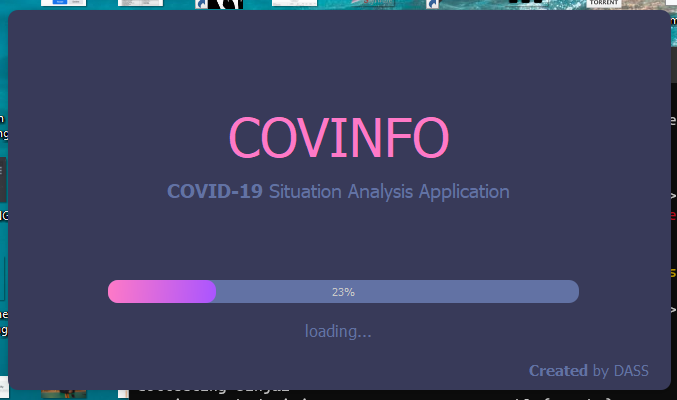
\includegraphics[width = 150mm]{SplashScreen.PNG}}
    \caption{Splash Screen}
\end{figure}
\clearpage
\thispagestyle{empty}
\begin{figure}[h]
    \centerline{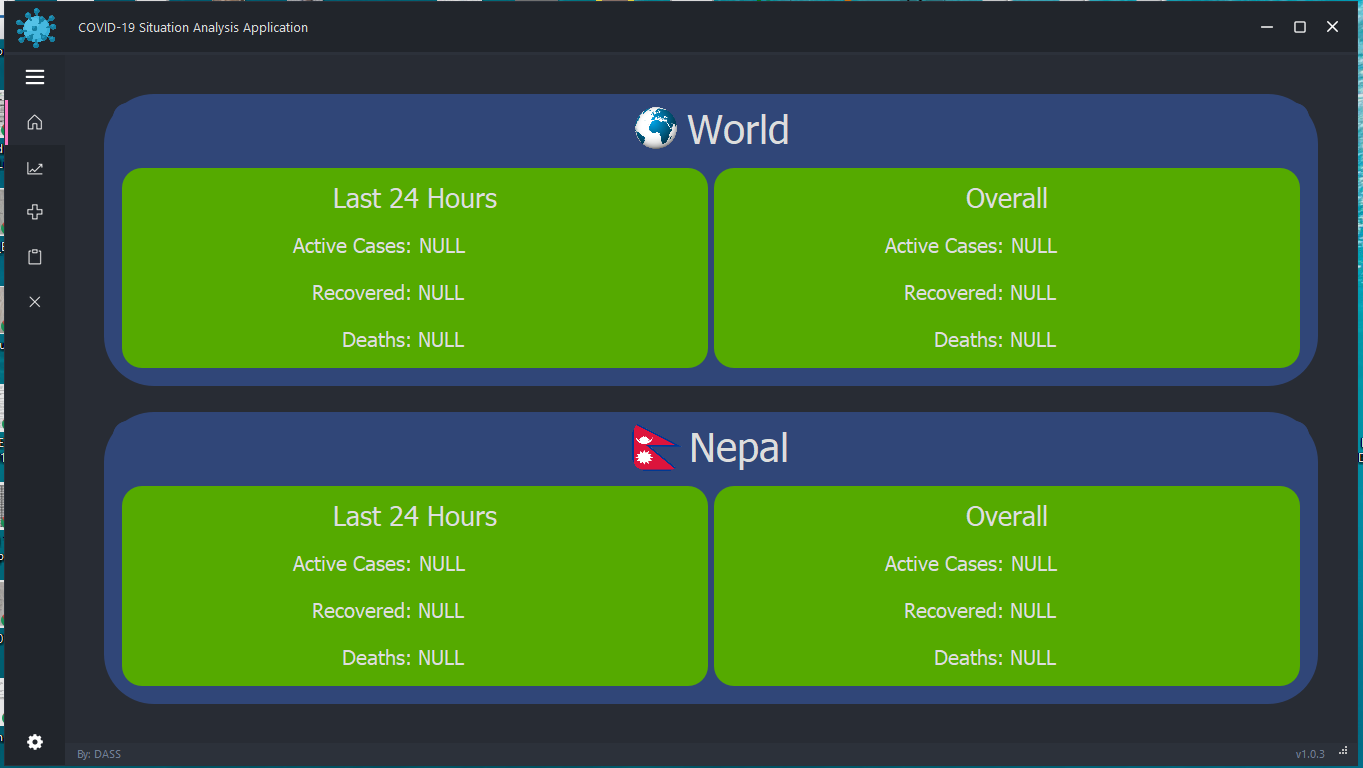
\includegraphics[width = 150mm]{MainWindowDashBoard.PNG}}
    \caption{Main Window - Dashboard}
\end{figure}
\clearpage
\thispagestyle{empty}
\begin{figure}[h]
    \centerline{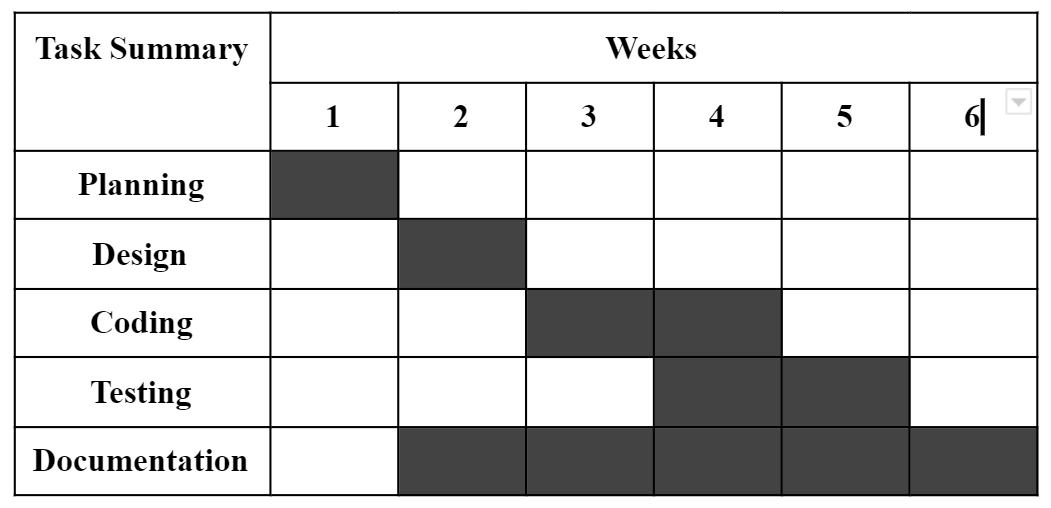
\includegraphics[width = 190mm]{chart.png}}
    \caption{Gant Chart}
    \label{fig}
\end{figure}
\rightline{\underline{\textbf{Index}}}
\begin{figure}[h]
    \rightline{
\includegraphics[width=15mm,height=15mm]{box.png}}
\end{figure}
\rightline{\underline{\textbf{Task Completed}}}

\end{document}
